\chapter{Hardware Accelerator}

The Raspberry Pi 5 with an Ai kit was chosen as the hardware to prove the concept of computing data at the edge.
This desiction was taken based on recommendations from the advisors and the avilability.
The market analysis confirms this choice.
The hardware accelerator of the Ai kit is made by Hailo \cite{hailo}.
Generally a hardware accelerator is used to compute neural netwroks like a graphics card is used to compute graphics.
Hailo is a company which produces hardware accelerators.
The Ai kit uses the Hailo-8L entry level hardware accelerator.
Hailo provides a pipeline to compile a network so that it can be executed on the hailo software.
First we take a look at the compilation of a network which has to be done on a PC, 
preferibly one with a GPU.
Secondly were looking on the way to run the network on the edge.

\section{Network compilation}
As sad before, the network has to be precompiled on a PC.
The application which is meant for this task is called the \Acrfull{dfc}.

\subsection{Dataflow compiler
\label{section:dfc}}

To use the \acrshort{dfc} a pytorch or tensorflow model has to be converted to Onnx or tensorflow light.
Information and pictures are taken from the Hailo Dataflow Compiler User Guide\cite{hailo_dataflow_compiler}.
The \acrshort{dfc} the compiles the model to a \Acrfull{hef} by executing the following steps:

\begin{enumerate}
    \item Full Precision Optimization
    \item Quantization Optimization
    \item Compilation
\end{enumerate}
In the full precision optimization step ONNX file first gets compiled into a \acrfull{har} file, a file type defined by Hailo.
This step also includes any changes to the model in the floating-point precision domain, for example Equalization\cite{meller2019same}, \acrshort{tse}\cite{Vosco_2021_ICCV} and pruning.

In the quantization optimization step the model gets compressed.
This means that the model gets converted from floating point to integer.
Weights get compiled to either 4,8 or 16 bits.
Activaitions get compiled to 8 or 16 bits.
Which quantisation is applied is handeled through a model script.
In that script the amount of quantized weights can be described.
There is also the posibility to target specific layer by the model script.
It is also possible to add preprocessing steps to the model script like resize the input or convert the input from RGB to YUV.
The result of this step is a quantized \acrshort{har} file.
This file can be compiled to a \acrshort{hef} file to use the model on Hailo hardware.

\begin{figure}[!h]
    \centering
    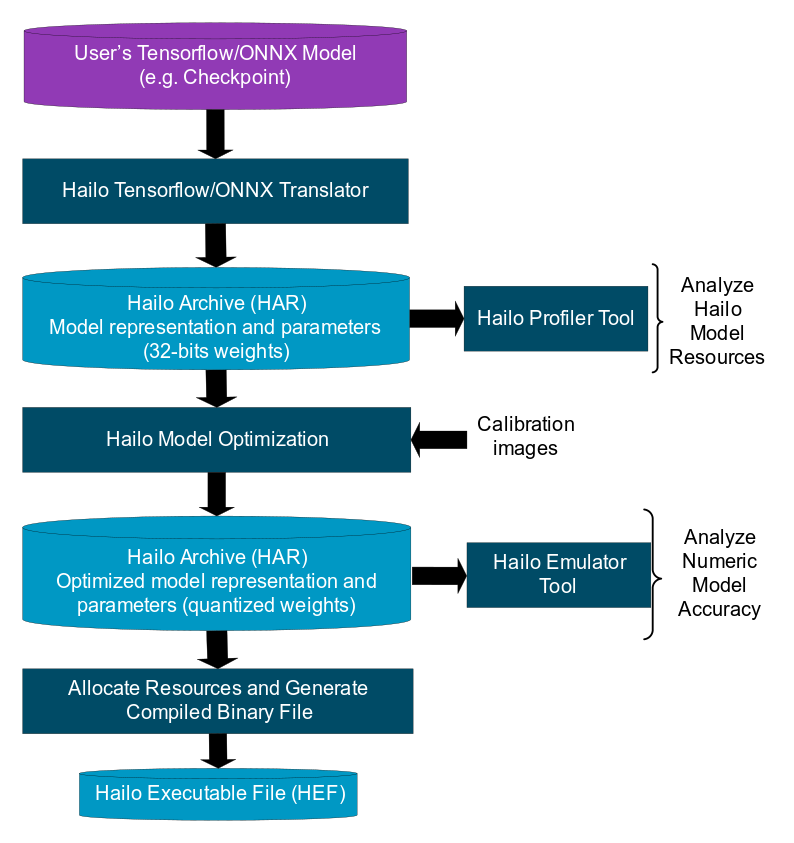
\includegraphics[width=\textwidth]{Images/Hardware/model_build_overview_with_onnx_and_hef_w_har.png}
    \caption{\Acrlong{dfc} overview \cite{hailo_dataflow_compiler}}
    \label{fig:hardware:dfcoverview}
\end{figure}

\subsection{Constrains}
At the time of this writing, the \acrshort{dfc} is not capable of compiling Transformers.
This is a very important limiting factor for this porject.
The best performance for CLIP is achieved with vision Transformers as image encoder.
Fortunately, the visual encoding of CLIP can also be done with ResNet, a special form of \Acrshort{cnn}'s.

\section{Running on the edge}

Hailo provides a library called TAPPAS which is based on GStreamer.
The library enables using a Hailo device within gstreamer pipelines t create intelligent video processing applications.
The information for this section are taken from the TAPPAS User Guide.
In the point of time there are two approaches to run a network on a hailo device.
One with Gstreamer and one with a Python API.
There are many different example applications available for many diffrent usecases.
These examples can be found in the Hailo model zoo\cite{hailo_model_zoo} or in their repo for Raspberry Pi examples \cite{hailo_rpi5_examples}.


\subsection{GStreamer approach}

Gstreamer is a framework for creating streaming media applications.
It enables the design any type of multimedia application but it isnt restridted to audio and video processing.
The framework can porcess any kind of dataflow.

GStreamer consists of blocks which can be concantenated.
To work with the Hailo hardware accelerator some blocks in the pipeline get offloaded to the Hailo processor.
A python programm is used to construct a string which then is executed in a terminal.
A example pipeline can be seen in \cref{fig:hardware:gstreamerpipeline}.
More examples with code can be found in the TAPPAS User Guide.
\begin{figure}[!h]
    \centering
    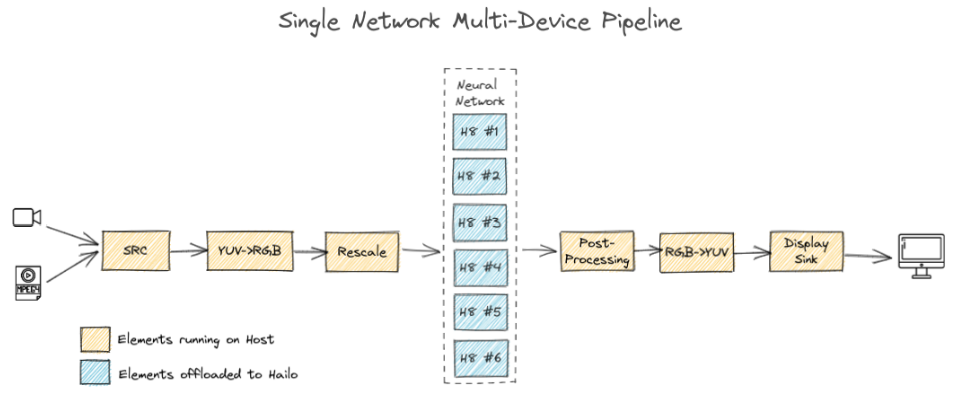
\includegraphics[width=\textwidth]{Images/Hardware/gstreamerExample.png}
    \caption{Example GStreamer pipeline from TAPPAS User Guide}
    \label{fig:hardware:gstreamerpipeline}
\end{figure}

\subsection{Python API approach}

With the Python API approch one can execute the whole inferance in python.
That makes the programm very simple in comparison to the GStreamer approach.
In python the Hailo hardware accelerator gets treated as an object with dedicated functions to use inference.
Importent to know is that hailo swaps the input dimension of the network.
This menas that the dimensions of the input to the network has to be adjusted.
Due to complexity of the GStreamer approch the Python API is used in this project.